%% Draft document mode
\documentclass[11pt,a4paper,bibtotoc,idxtotoc,headsepline,footsepline,footexclude,BCOR12mm,DIV13]
{scrbook}

%% Final document
%\documentclass[11pt,a4paper,bibtotoc,idxtotoc,headsepline,footsepline,footexclude,BCOR20mm,DIV10]{scrbook}

% KOMA-Optionen:
%  bibtotoc: include bibliography in table of contents
%  idxtotoc: include index in table of contents
%  headsepline: use horizontalline under heading
%  BCOR: binding correcion (Bindungskorrektur) (e.g.: BCOR5mm)
%  DIV: Number of sheet sections (used for layout) (e.g.: DIV12) 

%\makeindex
	%% inter line spacing
%\linespread{1.0}

% Set here the title, authors and other stuff to be used for the cover
% This file is used by MAIN.TEX

% set title, authors and stuff for the cover
\def\doctype{Master's Thesis in Informatics}
\def\title{Smart-home intrusion detection using network intrusion detection techniques}
%\def\title{Intrusion detection on the smart-home using network intrusion detection techniques}
%\def\title{Using network intrusion detection techniques to detect intruders on the smart home}
%\def\title{Network intrusion detection techniques on the smart home domain}
\def\titleGer{Einbruchserkennung in Smart-Home Umgebungen mittels Network Intrusion Detection Techniken}
\def\author{Manuel Munoz}
\def\supervisor{Professor Bernd Bruegge, Ph.D.}
\def\advisor{Stefan Nosovi\'{c}, M.Sc.}
\def\date{November 15, 2015}

% text to appear in the footer
\def\footertext{}
var OpenHAB = {}; // Settings object


//----------- PICTOGRAM ICONS -----------
// Set "usePictogramIcons" to true if PNG pictogram icons are used. Set to false if normal color PNG images are used as icons.

OpenHAB.usePictogramIcons = false;



//----------- UPDATES -----------
// Set "enableUpdates" to "true" if you want GreenT to check for new versions and updates itself, "false" to disable updates and "password" to enable updates only after a password is provided. You can set the password via "updatesPassword" setting.

OpenHAB.enableUpdates = 'true';


// Set "updatesPassword" with your desired password (only needed when OpenHAB.enableUpdates = 'password'). 
OpenHAB.updatesPassword = '123456';
% Commands to be used within the TUM report document
% Included by MAIN.TEX
% Please include your own cool commands here. 
% Be only sure to comment it sufficiently so others can use it.

%-------------------------------------------------------------
%                      Own Commands
%-------------------------------------------------------------


%-------------------------------------------------------------
% math stuff -------------------------------------------------

% nice R, N, C
\newcommand{\nat}{\mathbb{N}}
\newcommand{\real}{\mathbb{R}}
\newcommand{\compl}{\mathbb{C}}



% norm
\newcommand{\norm}[1]{\left\| #1 \right\|}

% un demi
\newcommand{\half}{\frac{1}{2}}

% parantheses
\newcommand{\parenth}[1]{ \left( #1 \right) }
\newcommand{\bracket}[1]{ \left[ #1 \right] }
\newcommand{\accolade}[1]{ \left\{ #1 \right\} }
%\newcommand{\angle}[1]{ \left\langle  #1 \right\rangle }

% partial derivative: %#1 function, #2 which variable
% simple / single line version
\newcommand{\pardevS}[2]{ \delta_{#1} f(#2) }
% fraction version
\newcommand{\pardevF}[2]{ \frac{\partial #1}{\partial #2} }

% render vectors: 3 and 4 dimensional
\newcommand{\veciii}[3]{\left[ \begin{array}[h]{c} #1 \\ #2 \\ #3	\end{array} \right]}
\newcommand{\veciv}[4]{\left[ \begin{array}[h]{c} #1 \\ #2 \\ #3 \\ #4	\end{array} \right]}

% render matrices: 3  dimensional (arguments in row first order)
\newcommand{\matiii}[9]{\left[ \begin{array}[h]{ccc} #1 & #2 & #3 \\ #4 & #5 & #6 \\ #7 & #8 & #9	\end{array} \right]}
%DOESN'T WORK,DON'T KNOW WHY \newcommand{\mativ}[16]{\left[ \begin{array}[h]{cccc} #1 & #2 & #3 & #4 \\ #5 & #6 & #7 & #8 \\ #9 & #10 & #11 & #12 \\ #13 & #14 & #15 & #16 \end{array} \right]}


%-------------------------------------------------------------
%-------------------------------------------------------------


%-------------------------------------------------------------
% some abreviations ------------------------------------------
\newcommand{\Reg}{$^{\textregistered}$}
\newcommand{\reg}{$^{\textregistered}$ }
\newcommand{\Tm}{\texttrademark}
\newcommand{\tm}{\texttrademark~}
\newcommand {\bsl} {$\backslash$}

%-------------------------------------------------------------
%-------------------------------------------------------------


%-------------------------------------------------------------
% formating --------------------------------------------------

% Theorem & Co environments and counters
\newtheorem{theorem}{Theorem}[chapter]
\newtheorem{lemma}[theorem]{Lemma}
\newtheorem{corollary}[theorem]{Corollary}
\newtheorem{remark}[theorem]{Remark}
\newtheorem{definition}[theorem]{Definition}
\newtheorem{equat}[theorem]{Equation}
\newtheorem{example}[theorem]{Example}
\newtheorem{algorithm}[theorem]{Algorithm}

% inserting figures
\newcommand{\insertfigure}[4]{ % Filename, Caption, Label, Width percent of textwidth
	\begin{figure}[htbp]
		\begin{center}
			\includegraphics[width=#4\textwidth]{#1}
		\end{center}
		\vspace{-0.4cm}
		\caption{#2}
		\label{#3}
	\end{figure}
}




% referecing figures

\newcommand{\refFigure}[1]{ %label
	figure \ref{#1}
}
\newcommand{\refChapter}[1]{ %label
	chapter \ref{#1}
}

\newcommand{\refSection}[1]{ %label
	section \ref{#1}
}

\newcommand{\refParagraph}[1]{ %label
	paragraph \ref{#1}
}

\newcommand{\refEquation}[1]{ %label
	equation \ref{#1}
}

\newcommand{\refTable}[1]{ %label
	table \ref{#1}
}




\newcommand{\rigidTransform}[2]
{
	${}^{#2}\!\mathbf{H}_{#1}$
}

%code, in typewriter
\newcommand{\code}[1]
 {\texttt{#1}}

% comment that appears on the border - very practical !!!
\newcommand{\comment}[1]{\marginpar{\raggedright \noindent \footnotesize {\sl #1} }}

% page clearing
\newcommand{\clearemptydoublepage}{%
  \ifthenelse{\boolean{@twoside}}{\newpage{\pagestyle{empty}\cleardoublepage}}%
  {\clearpage}}


%-------------------------------------------------------------
%-------------------------------------------------------------


\newcommand{\etAl}{\emph{et al.}\mbox{ }}

\makeglossary

\begin{document}

	\frontmatter
	% The front cover for the TUM report document.
% Included by MAIN.TEX


%--------------------------------------------------
% The Front Cover
%--------------------------------------------------

% The front cover for the TUM document.
% Included by MAIN.TEX


%--------------------------------------------------
% The Front Cover
%--------------------------------------------------

% correct BCOR - undo at the end !!!
\def\bcorcor{0.15cm}
\addtolength{\hoffset}{\bcorcor}

\thispagestyle{empty}

 \vspace{4cm}
\begin{center}
	       \oTUM{4cm}
	   
	   \vspace{5mm}     
	   \huge FAKULT{\"A}T F{\"U}R INFORMATIK\\ 
	   \vspace{0.5cm}
	 \large DER TECHNISCHEN UNIVERSIT{\"A}T M{\"U}NCHEN\\
    \vspace{1mm}
        
	\end{center}
		

\vspace{15mm}
\begin{center}

   {\Large \doctype}

  \vspace{20mm}
  
  {\huge\bf \title}\\%[3ex]
  
    \vspace{15mm}
  
  
  {\LARGE  \author}
  
  \vspace{10mm}
  
  \begin{figure}[h!]
  \centering
   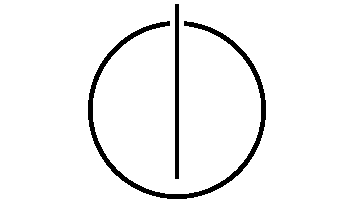
\includegraphics[width=4cm]{styles/informat.png}
  \end{figure}
  
  \end{center}
	\clearemptydoublepage
	% The titlepage for the CAMP report document.
% Included by MAIN.TEX


%--------------------------------------------------
% The title page
%--------------------------------------------------

% correct BCOR - undo at the end !!!
\def\bcorcor{0.15cm}
\addtolength{\hoffset}{\bcorcor}

\thispagestyle{empty}

 \vspace{10mm}
\begin{center}
	       \oTUM{4cm}
	   
	   \vspace{5mm}     
	   \huge FAKULT{\"A}T F{\"U}R INFORMATIK\\ 
	   \vspace{0.5cm}
	 \large DER TECHNISCHEN UNIVERSIT{\"A}T M{\"U}NCHEN\\
        
	\end{center}
		

\vspace{10mm}
\begin{center}

   {\Large \doctype}

  \vspace{10mm}
  
  {\LARGE \title}\\
  
  
  \vspace{10mm}
  
  
  {\LARGE  \titleGer}\\
  
  
  \vspace{10mm}

    %\hfill
    \begin{tabular}{ll}
	   \Large Author:     & \Large \author \\[2mm]
	   \Large Supervisor:    & \Large \supervisor \\[2mm]				
	   \Large Advisor:	& \Large \advisor \\[2mm]
	   \Large Date:       & \Large October 30, 2013
	 \end{tabular}
	 
	 \vspace{5mm}
	 
	 \begin{figure}[h!]
  \centering
   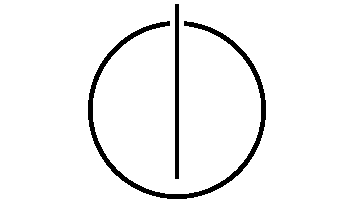
\includegraphics[width=4cm]{styles/informat.png}
  \end{figure}
   

\end{center}

% undo BCOR correction
\addtolength{\hoffset}{\bcorcor}
	\clearemptydoublepage


\thispagestyle{empty}
	\vspace*{0.8\textheight}
	\noindent
	
	I assure the single handed composition of this master's thesis only supported by declared resources.
	
	\vspace{15mm}
	\noindent
	Munich, Germany, 2013-10-31 \hspace{5cm} \author
\newpage
	\clearemptydoublepage
\phantomsection
\addcontentsline{toc}{chapter}{Acknowledgements}	


%\chapter*{Acknowledgements}

\vspace*{2cm}

\begin{center}
{\Large \bf Acknowledgments}
\end{center}

\vspace{1cm}


Many have sported me one way or the other to while writing these thesis. If I fail to mention your name, it is does not represent how grateful and lucky I am for having your support. 

I would specially like to thank my adviser Stefan Nosovi\'{c}. His constant support, encouragement, and willingness to discuss ideas greatly helped me during the process of writing my thesis. I also would like to thank Professor Bernd Bruegge for the chance to develop this work in the chair of the university that I believe to be the coolest. Furthermore, his feedback greatly enhanced my understanding of the problem at hand.

I also would like to thank my family in my mother tongue. If you do not understand Spanish, please do not take it personally. The gist of it is that they are awesome and I could not be here without them.\\
A mi familia muchas gracias por todo el apoyo que me han brindado desde la distancia. Sus constantes palabras de \'{a}nimo y sobretodo su ejemplo de perseverancia, han influido mucho la persona que soy hoy en d\'{i}a. 

	% Abstract for the TUM report document
% Included by MAIN.TEX


\clearemptydoublepage
\phantomsection
\addcontentsline{toc}{chapter}{Abstract}	

\vspace*{2cm}
\begin{center}
{\Large \bf Abstract}
\end{center}
\vspace{1cm}


In recent years we have witnessed increasing interest in smart environment from researches, and from the public, about smart homes. The appliance industry has noted this interest and also has increased the number of products geared towards home automation.
These products take advantage of wireless communication technologies to monitor, and in some cases autonomously control the environment they are in. Through their interaction and collaboration, they can make spaces more comfortable and more secure. Nevertheless, the alternatives for smart home security are not yet appealing. In order to be attractive to the general consumer, they have to outperform the traditional security systems. 

One of the problems facing traditional home security systems, is the issue of false positives. A false positive, in the context of the home, is defined as reporting an intrusion or a burglary when really nothing has occurred. We developed a system that aims to reduce the occurrence of false positives, while detecting security anomalies. To that effect, we explored the available research and existing algorithms from the networking discipline, which has dealt with intrusion detection since the 1960s. 

We aim to address these issues with the development of Rosie, a system that collects and analyses data from sensors, in order to recognize usual behavior of the inhabitants of the home, and distinguish it from abnormal behavior. 

Rosie, also serves as a platform for studying new intrusion detection algorithms, by providing simple ways of extending the software. As a proof of concept, the system uses algorithms from network intrusion detection systems. These techniques analyze communication, temporal patterns of the network traffic loads, and the content of the packets. The same type of information can be found in smart environments, and is therefore useful for distinguishing usual and unusual behavior of inhabitants.


	\tableofcontents
  	\clearemptydoublepage

\phantomsection
\addcontentsline{toc}{chapter}{Outline of the Thesis}

\begin{center}
	\huge{Outline of the Thesis}
\end{center}

%--------------------------------------------------------------------

\noindent {\scshape Chapter 1: Introduction}  \vspace{1mm}

\noindent  The introduction starts with a motivation by describing the current challenges of ... \\

\noindent {\scshape Chapter 2: Requirements Elicitation}  \vspace{1mm}

\noindent  Chapter 2 describes the requirements elicitation which includes the scenarios that drive the development of this project. Based on these scenarios, non-functional requirements are proposed and a functional model with use cases and functional requirements is elaborated. \\

\noindent {\scshape Chapter 3: Analysis}  \vspace{1mm}

\noindent  Chapter 3 describes an analysis model based on the requirements. The model is created to formalize the objects and information that exist in the domain of ... \\

\noindent {\scshape Chapter 4: System Design}  \vspace{1mm}

\noindent  Chapter 4 describes the system design model which contains ... \\

\noindent {\scshape Chapter 5: Object Design}  \vspace{1mm}

\noindent Chapter 5 describes ...
Afterwards, the transformation of application domain objects to solution domain objects is discussed. \\

\noindent {\scshape Chapter 6: Conclusion}  \vspace{1mm}

\noindent  Chapter 6 concludes with an overview of the results. Afterwards, the results are reviewed critically and visions for future work are pointed out. \\


	
% ---------------------------------------------------------------------------
%
% 	Thesis Main Part
%
% ---------------------------------------------------------------------------

\mainmatter
\chapter{Introduction}
\label{chapter:Introduction}

\section{Problem Statement}

Recent years have seen the increase of interest in smart homes\cite{googletrends}. The number of products geared towards smart homes has also increased, as it can be seen at trade shows like CES\cite{cnet}. Big manufacturers of consumer electronics have reacted to this trend, and have launched product lines aimed towards that market segment. These products take advantage of wireless communication technologies to control and monitor the environment they are in. The impact of integrating these products into everyday life can enable new ways of interacting with the environments, making them more comfortable, or even more secure.

\subsection*{Problem}
According to the statistics gathered by the German police, 2014 saw the highest number of break-ins in 16 years. In comparison with the previous year, there was a 2\% increase of break-in cases\cite{breakins}. These increasing numbers make the people feel less safe in their own homes.

The best known method to secure a household is to hire a security company to provide, install, and also monitor a security system. When a sensor of the security system is triggered, the security company is notified, and can alert both the authorities and the user. \\
However, this approach has some drawbacks. The installation of the system comes with a price, because it involves breaking the walls to hide cables and panels that are used to control the system. In order to monitor the household, the security company has access to the the security system, which may raise user's privacy concerns. When the system is triggered, the security company reacts by contacting local authorities or the user. Different events such as pets, can trigger the system resulting in a waste of resources.

One way of tackling some of the existing drawbacks of current security systems, is to take advantage of the increasing ubiquity of smart sensors present in smart spaces. By collecting and analyzing data from smart sensors, it is possible to recognize the usual behavior of the inhabitants of the household \cite{behavior}, and separate it from the unusual\cite{anomaly}. 

Registering, recording, and analyzing data from different users, in order to identify unusual and potentially harmful behavior has been used on networking systems for a long time, and some of the concepts and ideas may be find a parallel on the smart home.

\subsection*{Proposed Solution}
Unusual behavior of network users can be recognized using network intrusion detection systems. These systems analyses communication the temporal patterns of network traffic loads and the content of the payload. The same type of information can be found in smart environments. In this thesis, we would like to explore the possibility of applying existing network intrusion detection techniques in smart home environment, with a goal of detecting unusual behavior of inhabitants. Special focus will be set on burglary detection scenarios.

%As a part of this thesis, we foresee the development of a software infrastructure that will enable us to compare the performance of different algorithms used in network intrusion detection systems. The architecture of the software will have to enable simple ways of extending the software with new intrusion detection algorithms. Our software will have to support seamless integration with the existing OpenHab framework.


\section{Related Work}
\label{related_work}

%The Aware Home, Georgia Tech University
\textbf{Kidd \etAl, 1999: The Aware Home: A Living Laboratory for Ubiquitous Computing Research} \cite{raey} \\
This project from the Georgia Institute of Technology, was created as "a living laboratory for interdisciplinary design, development and evaluation"\cite{Kientz:2008:GTA:1358628.1358911}. The objective of the project was to provide a platform where different disciplines could test their hypotheses regarding new technologies for the home environment. The team at the Georgia Institute of Technology built a three-stories house and equipped it with sensors that captured and registered almost every event that happened around the house, using pinhole cameras, microphones, voltmeters, etc. The applications here developed target specific scenarios like supporting aging in place, and supporting busy families. \\
The first scenario addresses problems that stay-at-home senior citizens may have. Issues such as safety, accident prevention and detection, aid in daily activities (reminders and familiarization with new technologies), and facilitating communication with the outside. For example, the project \textbf{Memory Mirror}\cite{Kientz:2008:GTA:1358628.1358911} identifies the objects used by the resident, and post them on a mirror creating a reminder. In the case the user has interacted with the object before, the mirror posts usage statistics.
The supporting busy families scenario is targeted to households where parents work but also need to take care of another family member. The issues include household schedule maintenance, care for individuals with special needs, and make life more enjoyable. The \textbf{Baby Steps} \cite{Kientz:2007:GKU:1240624.1240830} project tracks and logs milestones on the baby's cognitive development cycle, that way if a milestone is missed, the house can provide additional time line information to the doctors.\\
The project from the Georgia Institute of Technology is a good example of what it can be done, when a living space is designed and built as a smart space from the ground up. The house was thought from the start to have a large set of sensors. For example, for activity recognition the Aware Home has 10 pin-hole cameras in just one room\cite{Kientz:2008:GTA:1358628.1358911}. Our project is focused on living spaces that already exist, and it is not possible to install a high number of sensors.\\
From the applications point of view, none of the Aware home project projects tackle the problem of home security or intrusion detection. However, machine learning algorithms are used for activity identification.\\

%MavHome, University of Texas at Arlington
\textbf{Cook \etAl, 2004: MavHome: an agent-based smart home} \cite{1192783} \\
The University of Texas at Arlington proposed an architecture to model the home as an rational agent. It uses sensors to measure what happens on a home, and then uses different actuators to modify it's state. MavHome proposes an architecture that allows the home to learn the behavior of the inhabitants and interactions they have with the home. The agent uses a layered architecture\cite{1192783} with 4 layers. The physical layer communicates the system with the hardware components of the house. The communication layer transmits the data between agents. The information layer is responsible to gather, store, and generate new knowledge that is going to be used on the decision-making process. The decision layer takes the knowledge provided by the information layer and selects actions to be executed. The decision layer has prediction algorithms take sequence of interactions between the inhabitant and the home, and then compares it with previously stored sequences in order to predict the next possible actions. However, the events that can be automated are the ones that occur with certain frequency. \\
To test the project the University also built two physical spaces and a simulation space\cite{inhabitantguidanceofsmartenvironments}. The first space from the physical ones, is a workplace environment equipped with work areas, cubicles, a break room, lounge, and a conference room. The second space is completely equipped apartment. The project also counts with a simulation tool that allows to the machine learning algorithms to be trained, to be later deployed on the physical environments.\\ 
The project arrived at one conclusion that is of importance our hypothesis. Machine learning algorithms can be used to "model and predict inhabitant activities, and that a policy can be learned using this information to automate a smart environment"\cite{inhabitantguidanceofsmartenvironments}.\\

%The Adaptive House, University of Colorado at Boulder
\textbf{Mozer, 2004: Lessons from an adaptive house}\cite{mozer2004lessons}
The Adaptive Home is a project for the University of Colorado at Boulder. It started 1996 with the idea that smart homes should not provide a different control interface, from the one that users normally use. The house uses machine learning algorithms to control heating, ventilation, air conditioning systems, the water heater, and lighting. The Adaptive Home, after observation of the interaction between the house and the users, can deduct patterns and make predictions. If the users are not happy with the predictions, they can change the values selected by the house using the normal interface. The main objective of the Adaptive Home is comfort while reducing operating costs\cite{mozer2004lessons}.\\
The algorithm uses two constraints that need to be optimally satisfied: cost and discomfort. Through reinforcement learning, it is possible to calculate the next action for the current state, or for the next predicted state. Coarse activity identification is also one of the main focuses on the project. Once an activity is identified, the system can trigger an event that in turn will change the state of the house\cite{mozer2004lessons} into the predicted one.\\
This project not only boosts the idea from using machine learning on the home environment, but also provides an interesting perspective to that aspect, because it includes the discomfort constraint. The system calculates the cost of performing an action, not only with monetary value but also with how annoying the action can be if it is wrong. It is also interesting that it does not discretized time into timed intervals, but into event changes that trigger states changes.\\
For this project security of the smart home was not explored. However, the use of machine learning algorithms support the idea that it is possible to do activity identification, and execute actions according to those states. \\

%Aire project: Focuses on work spaces

%CyberManor, Internet Home Alliance. Company, not a Uni project
%CASAS Smart home project. Data sets MavHome comes from them.
%EasyLiving, Microsoft
%Hal, MIT Artificial Intelligence Laboratory. No home automation project
%Home Automation, IBM

%House_n, MIT
\textbf{Intille, 2004: The Goal: Smart People, Not Smart Homes} \cite{smartpeople} \\
The Massachusetts Institute of Technology also decided to explore the smart home with a multi-disciplinary approach. Many industry partners and other departments at MIT co-founded the House\underline{ }n project. The goal of this project \cite{smartpeople} was to shift the investigation's focus from a smart home that automates all possible activities, to one where the smart home requires user's interaction to help maintaining life stimulating.\cite{smartpeople}.\\
Within the House\underline{ }n project, MIT joined forces with industry partners used the approach of building a live-in laboratory. There, volunteers would move in for a period of time and lead their lives normally, while also being measured by many sensors. The laboratory was built in 2004 and it is called the PlaceLab\cite{placelab}. 
The focus of this project\cite{placelab} was proactive health care. By providing relevant, just-in-time information\cite{dietary} the home influence the occupants to make better dietary choices. Also, the project focuses on the influence of technology can impact independence of aging seniors\cite{aginginplace}, using different methods of indoor positioning\cite{bhack}, and the implications of user tracking\cite{info:doi/10.2196/jmir.8.4.e29}. All other projects tackled problems from other disciplines like material engineering and architecture.\\
%IIB, Trinity College Dublin
%i-LAND, Ambiente
%Interactive Workspaces, Stanford University. collaborative work settings
%Neural network house from 1995. May be too old.
%PRIMA, Inria
%The intelligent home 1999. May be too old.
%Smart Spaces Lab, NIST. Project for working spaces detecting meetigns 
%SMART Connected Home, GE

%Machine learning 
\textbf{Fung \etAl, 2013: Intrusion Detection Networks: A Key to Distributed Security} \cite{fung2013CRC} \\
Intrusion detection systems are designed to monitor all the elements deployed on a network, and alert in case out of the ordinary behavior is detected. Network intrusion detection techniques can be divided into two: Signature-based and anomaly-based\cite{fung2013CRC}. Signature-based techniques use a predefined list of already identified intrusion methods, and compares the network's traffic to filter out possible intrusion attempts. Anomaly-based techniques compare the behavior of the network with a precollected baseline of normal behavior. This technique is the one we want to explore with our current work, under what circumstances anomaly detection can be extended to the smart environment, and which of the intrusion detection methods can be also used on the home.\\
 
\textbf{Bhattacharyya \etAl, 2013: Network Anomaly Detection: A Machine Learning Perspective} \cite{Bhattacharyya:2013:NAD:2505468} \\
The work of Bhattacharyya \etAl analyzes thoroughly the different machine learning techniques used on anomaly-based network intrusion detection. According to the authors, it is possible to analyze the traffic on a network, and then classify it between malicious or normal behavior. This characteristic turns the anomaly detection problem into a classification problem\cite{Bhattacharyya:2013:NAD:2505468}.\\
The authors also present a list of requirements that must be met by real-time or near real-time systems, that can be adapted to the smart home environment: 
1) These systems must detect anomalies with high detection accuracy with minimal or even no prior knowledge of the environment, and also must observe that environment and learn what is the normal behavior of it. 
2) The identification process must be done with the minimum amount of false positives. 
3) The number of features should be the least possible. The authors also propose other two requirements, which they are implicit to the smart environment.

The work of Bhattacharyya \etAl also categorizes the machine learning techniques used for network anomaly detection into six categories. 
	\begin{itemize}
		\item \textbf{Supervised learning}
		
This method assumes that it is possible to start with a batch of labeled data called a training set. This collection of data is used to build a model, to which all new data can be compared against and decide if the behavior is normal or not. This categorization is divided into parametric and nonparametric methods. \\
The first approach assumes that the data is produced using a parametric distribution and probability density function.
The second approach, the nonparametric method, does not start with a model but creates one from the data. The most used nonparametric method for anomaly detection is to take the training set and create a function that maps the date to the interval from [0,1]. Then, a data point is evaluated with that function, and if it scores under a certain predefined threshold then is considered anomalous.\\
One of the advantages of using supervised learning is that if the system runs for long enough, it is possible to establish a very good baseline to be used as a comparison. The disadvantages include susceptibility to being trained to consider as malicious traffic as normal. Also, due to the assumptions made by the model and on the grounds that setting all the parameters is very difficult, the ratio between false positives and false negatives is unfavorable. The disadvantages seem to outweigh the advantages.\\

		\item \textbf{Unsupervised learning}
		
For supervised learning it is very important to have labeled data. However obtaining that data may be very difficult or expensive, since the use of experts is needed. Methods that do not rely on labels are called unsupervised, and they may be better suited to set the baseline that represents normal behavior. \\

One of the methods is \textit{clustering}. Here a representative point is selected for each desired cluster, then each test data point is taken, and classified according to the nearest cluster. Here the disadvantage of an expert becomes again apparent. However works like UNADA\cite{unada} where Casas \etAl{} introduced a clustering algorithm for unsupervised network anomaly knowledge-independent detection of anomalous traffic. This algorithm uses a clustering technique to identify clusters and outliers in multiple low-dimensional spaces.\\

%needs explanation of how it works and how it can be translated to smart homes
\textit{Association mining} tries to identify events that happen together. This technique assumes that patterns in the data can be identified. Typical usage of association mining, is when stores perform market research to better stock their shelfs, analyzing the data it is possible to come interesting conclusions. For example, customers from a convenience store that buy product A always end up buying also product B on the current or future visits. With that sort of information the market can stock product A and B together. That is way some stores set aside shelf space for lemons on the alcoholic beverages aisle. Intrusion detection algorithms such as ADAM\cite{Barbara:2001:ATE:604264.604268} use this principles to identify out-of-the-ordinary behavior. \\

\textit{Outlier mining} takes the opposite approach of clustering. Here the techniques search for the data points that do not represent the majority of the data. This points are called outliers. These methods are distance-based, density-based
and soft computing approaches. The first one defines a function that measures the distance of the new data point in comparison to the training set. The selection of this function depends on the assumptions made on the data\cite{Gogoi:2011:SOD:1971494.1971504}. Density-based methods estimate the density distribution
of the data instance and then identify outliers as
those who are located in regions of low density\cite{Koufakou:2010:FOD:1743225.1743230}.\\

		\item \textbf{Probabilistic learning}
		
The techniques grouped by probabilistic learning allow for including random behavior or with probabilistic uncertainty. According to  Bhattacharyya \etAl the main characteristic of these techniques is they allow to "update previous outcome estimates by conditioning them with newly available evidence"\cite{Bhattacharyya:2013:NAD:2505468}. This seems like a desirable attribute to have, when evaluating human behavior, where probabilistic uncertainty us inherent.\\
%Hidden Markov Model based methods. 

\textit{Bayesian networks} is a model where the relationships between random variables are represented. Usually a direct graph is used in order to represent the random variables and the dependency relation between them. On the nodes of the graph also are incorporated the possible states of the random variable, and the conditional probability table\cite{Kruegel:2003:BEC:956415.956436}. The relation that the arcs exhibit is one of causality, that means that the child node is causally dependent of the parent nodes.\cite{Kruegel:2003:BEC:956415.956436}. \\
Kruegel \etAl explain in \cite{Kruegel:2003:BEC:956415.956436} that given the assumptions made with Bayesian networks, it is very likely to have a high number of false alarms, when used on network intrusion detection methods. Given the low probability of the parent variable, e.g. "an intrusion is occurring", and the dependence of the child's variable probability on the parents probability., e.g. "a motion sensor is tripped given that an intrusion is occurring".  \\

\textit{Hidden Markov models} is a mechanism to assign probability distributions to a sequence of observations at equally-spaced time intervals. Even thought this is a type of Bayesian network, they differ due on some of the extra assumptions that are made\cite{Ghahramani:2001:IHM:505741.505743}. The process is called \textit{hidden} because the observations are caused by states which are hidden to the observer. The other assumption is that the Markov property is fulfilled, that means, the current state is independent from all the past states. Also, implies that the current state contains all the information of the past states needed to calculate any future states. Bhattacharyya \etAl estate that it is possible to train the models by using data obtained by doing packet inspection, as well as system calls and commands.\\

\textit{Naive Bayes} based techniques have been also used on this field. Naive Bayes methods are a simplified version of the Bayesian network model\cite{Langley:1992:ABC:1867135.1867170}. Here, independence between the variables is assumed. That way, it is possible to calculate the a posteriori probability of an outcome given the a priori observations. Bhattacharyya \etAl and Kruegel \etAl note that there are however some limitations to the use of this technique. First, the assumed independence between the variables gives it the same classification capability as other simpler techniques, like threshold-base systems. Second, adding new information problematic. \\

\textit{Gaussian mixture model} based techniques are also used. This approach also assumes independence between the variables, however it uses Gaussian probability distribution functions to build the probability distribution each individual variable. This functions are called Gaussian mixtures. Bahrololum \etAl \cite{Bahrololum2008} developed an anomaly detection system using Gaussian mixture models. There, they use maximum likelyhood estimation to estimate the parameters of the Gaussian mixture model. Once the models were set up, they where trained using a famous dataset, which included instances of different network attacks, such as probing, denial-of-service, unauthorized access to local super user (root) privileges, and unauthorized access from a remote machine\cite{Bahrololum2008}. \\

%EM Model		

		\item \textbf{Soft computing}
		
		
Soft computing can be view as the opposite of traditional computing that requires a precise, even ideal, established analytical mode. Soft computing much like the human mind is tolerant of imprecision and uncertainty. This techniques often do not find exact solutions, and that makes them suitable for network anomaly detection.\\

The \textit{Genetic algorithms} approach represent a problem on a data structure much like chromosomes. Then, operators, like selection, recombination, and mutation are applied in order to generate new sample points in a search space\cite{geneticAlgos}. 
In the context of network anomaly detection, the chromosomes represent attributes like services, flags, number of super user attempts\cite{Bhattacharyya:2013:NAD:2505468}. \\	
Balajinath \etAl propose a network anomaly intrusion detection system based on genetic algorithms. This algorithm continuously captures and learns the user behavior in order to identify when that behavior is abnormal.  \cite{Balajinath:2001:IDT:2294491.2294970} Each command of the user forms a gene, and together with a fitness function calculated for a set of genes, new iteration of genes are computed to determine the probability of commands being intrusive.\\

\textit{Artificial neural networks} can also be used for anomaly and network intrusion detection. Neural networks are motivated on how fundamentally different the human brain and a computer process and compute information. The hierarchical multi-layered structure is composed of interconnected processing elements working in conjunction to solve specific problems. ANNs are commonly used on various applications such as data clustering, feature extraction and anomalous pattern identification.\\
The work by Lee \etAl\cite{935046} present a very interesting approach to network intrusion detection. They use a hierarchy of back propagation neural networks to detect in real time known and unknown attacks. Each neural network instead of being built with network data, they are built with the normal behavior contained on the TCP protocol.\\

\textit{Rough Sets} introduced by Zdzislaw \cite{Pawlak199748} deals with sets that include vagueness in its definition. The opposite are traditional sets also known as crisp sets. On a crisp set all the mathematical notions must be exact. On the other hand, rough sets define a boundary region, a lower approximation, and an upper approximation. The lower approximation consists of all objects which surely belong to the set. The upper approximation contains all objects which possibly belong to the set. Objects that cannot be classified with certainty as members of the set completely. The difference between the upper and the lower approximation constitute the boundary region of the vague concept.
Rough Sets  methods have been also researched as techniques for intrusion detection. Bhattacharyya \etAl explain that these techniques are useful on network intrusion detection because of their simplicity, and because they allow learning with small training datasets\cite{Bhattacharyya:2013:NAD:2505468}. Rough Sets have been used on network intrusion detection systems in conjunction with another techniques like fuzzy set theory \cite{4509827} and support vector machines\cite{5176039}.\\


Boolean logic is the one used by computers where the state of all elements can only be true or false. In \textit{fuzzy logic} that set is opened to more possible values. For example, when talking about the weather one can say that today the weather is great, good, ok, bad, or awful. An algorithm was develop by Dikerson \etAl to use fuzzy logic and statistics to identify network anomalies\cite{877441}. After a learning phase, ranges for the types of data being monitored are evaluated. Five fuzzy sets LOW, MEDIUM-LOW, MEDIUM, MEDIUM-HIGH, and HIGH, where determined to apply the same fuzzy rules to all the network input. Tajbakhsh \etAl also applied this concept to network intrusion detection. They extracted a set of fuzzy association rules for different classes, and is used as a model for each class. To determine the class of a set of transactions, they generate a set of fuzzy association rules from this transaction set and compute the similarity of the extracted rule set with sets mined from each class\cite{Tajbakhsh2009462}. The fuzzy association rule sets are used to describe normal and anomalous classes. A sample is considered normal if the compatibility of the rule set generated is above a certain threshold. Those with lower compatibility are regarded as anomalous.

A fuzzy class association rule mining method based on \textit{genetic network programming} was presented by Mabu \etAl. GNP is similar to genetic algorithms, but instead of strings to denote genes it uses directed graphs, which boosts the representation capability and node's reusability in a graph structure. Using both fuzzy set theory with GNP, this method can use discrete and continuous values to extract important class-association rules that boost detection ability\cite{5499108}.

%Xian et al. [388] propose a novel unsupervised fuzzy clustering method based on clonal selection for anomaly detection. The method is capable of obtaining global optimal clusters more quickly than competing algorithms.

\textit{Human Immune systems} have been also used to model algorithms called artificial immune systems. The objective of the human immune system is to recognize anomalies within the body. The immune system classifies some external objects that enter the body as undesirable and creates antibodies to fight those antigens. The process of identifying the antigens is called negative selection. This process has been used as motivation to develop network intrusion detection algorithms \cite{ais}, however the outcome is that the time need to create all the detectors to achieve high confidence is impractical for high dimensional data.


%		\item Knowledge-based  
%		
%		
%Rule based and Expert System based
%
%Ontology and Logic System based

		
%		\item Combination learners
%		
%		
%Ensamble based
%
%Fusion based
%
%Hybrid
		
	\end{itemize}


\section{Terminology}

The following section introduces definitions of ambiguous words that are used continuously throughout this thesis. 

\begin{itemize}

\item \textbf{Data point} 

\item \textbf{Training set} 

\item \textbf{smart environment} 


\end{itemize}


\chapter{Requirements Elicitation}
	
The present section will identify the actors that interact with our system. A description of the features from the point of view of the actors is given. With that description in mind, the use cases for the system's functionality is defined. Also, the restrictions over the system will be determined. The methodology of scenario-based requirements elicitation as defined by Br{\"u}gge \etAl on \cite{Bruegge2004} will be followed.
%In requirements elicitation, ...
%The requirements are gained from the scenarios described below. In general, requirements are divided into functional requirements referring to "interactions between the system and its environment independent" \cite{Bruegge2004} and non-functional requirements referring to "user-visible aspects of the system that are not directly related with the functional behavior". \cite{Bruegge2004} Pseudo requirements are constraints that were imposed by the client. The proposed intuitive control system is created on the assumption of the requirements elicitation described in the following sections.

\section{Scenarios}
\label{scenarios}


To have a better understanding of what a potential user may encounter every day when interacting with the system, a set of visionary scenarios where are devised, and are described below. \\

\textbf{Scenario 1: "Normal week day"} \\
\textbf{Participating Actor instances:} George:User, Jane:User, Judy:User, ROSIE:System \\
It is a weekday morning and George's family wakes up to start the day. Jane goes to the kitchen to get breakfast ready, and opens a window on the way. ROSIE notices that windows are being opened, and movement is being detected on the way to the kitchen. George and Jane go to work leaving Judy to get ready by and go to school. ROSIE detects that the doors are being opened, and George's and Jane's presence are not longer detected. ROSIE detects opening and closing of the doors, and the presence of Judy on the house. ROSIE recognizes that the activities are performed by authorized members of the household and maintains a the threat level as normal. On this level ROSIE is instructed to silently record the data, and to not dispatch any notifications.\\
Judy finally leaves the house to go to school. ROSIE detects that Judy's presence is no longer on the household and that from that point on any physical interaction with ROSIE should be considered abnormal. The threat level is raised to elevated. As per George configuration, ROSIE keeps recording sensor data, and also sends notifications in case anything abnormal is detected. \\

\textbf{Scenario 2: "Short day at work"} \\
\textbf{Participating Actor instances:} Jane:User. ROSIE: System\\
Jane was not feeling well at work and decided to go home early. As she gets home, ROSIE is in a elevated threat level detects that there is movement that is not typical for the hour and day. However, the system detects the presence of one of the authorized members and reduces the thread level to normal \\

\textbf{Scenario 3: "Who are you?"} \\
\textbf{Participating Actor instances:} Judy:User, ROSIE:System\\
Judy came from school, but as is usual she spent the whole day listening to music on her phone and the battery is dead as she came tho her empty home. ROSIE as it finds itself in a elevated threat level has the camera on and is scanning for familiar faces. ROSIE detects that there is a presence on the household, but cannot detect that it is an authorized user. To let ROSIE know that she is one of the authorized users she stands before the camera, and ROSIE recognizes Judy and reduces the threat level to normal.  \\

\textbf{Scenario 4: "A helping hand"} \\
\textbf{Participating Actor instances:} George:User, Henry:Unauthorized, ROSIE:System\\
On the day the hot water meter is scheduled to be read, neither George, Jane, nor Judy are at home to open the door to the person that reads the meters. Jane kindly asks the landlord Henry, to open the door of the house so the task can be completed. ROSIE detects the door being opened but distinguishes no authorized presence. The threat level is raised to exceptional, where the system monitors that the sensors that are outside the area where the meter is located are not tripped. That would mean that the temporally allowed users have entered an unauthorized area. \\
%On the day the hot water meter is scheduled to be read, neither George, Jane, nor Judy are at home to open the door to the person that reads the meters. Jane kindly asks the landlord Henry, to open the door of the house so the task can be completed. ROSIE detects the door being opened but distinguishes no authorized presence. The threat level is raised to exceptional, where notifications keep George updated, as well as the camera is turned on to check when the two men leave the house. Once they do, George can set the threat level back to elevated. \\

\textbf{Scenario 5: "Finally vacations"} \\
\textbf{Participating Actor instances:} ROSIE:System\\
The complete family takes a vacation for a couple of days. ROSIE detects that no authorized users are at home and it enters the elevated state. At this point ROSIE mimics the behavior with the actuators available. For example, the lights on the living room turn on at around 19.00, like they usually do when the family is there. \\

\textbf{Scenario 6: "Uh-oh"} \\
\textbf{Participating Actor instances:} George:User, Burglar:Unauthorized, ROSIE:System\\
On a normal week day, when all the family members are away attending to their responsibilities, a burglar decides to break into their home. Because no one is at home, ROSIE's threat level is set to elevated. The burglar finds a window that he can easily open, the system register this event and notifies George. As he receives the notification, he can to call the police and have them catch the thief. \\

\textbf{Boundary Scenario 7: "Initial Configuration"} \\
\textbf{Participating Actor instances:} George:User, ROSIE:System\\
George has recently acquired ROSIE. To use the features he needs to do some initial set up. First of all, he needs to train ROSIE with the faces of the trusted users. Second, he needs to configure the different available reactions to be executed when the threat level changes, e.g. turn the camera when the level is elevated.
%Ms. Cooper has moved to a new office and wants to set up HomeGestures for the first time. The administrator has already set up her room with its addressable fixtures on the server using a simple configuration file. \\
%Ms. Cooper opens the HomeGestures app on her iPhone. As her room is yet unknown, the device estimates her position in an adjacent room. She corrects this in the configuration tab by changing the room manually. The system is now taking WiFi measurements (called fingerprints) in the background. Ms Cooper chooses the "Learn fixtures" option and sees all addressable fixtures in her room by the given names of the administrator. She chooses her desk light first, points the iPhone to the light and presses the big button with the "Learn" caption. The app confirms with a sound and Ms. Cooper proceeds analogously with her other fixtures. The office is now configured and can be controlled by any authorized device.

\section{Functional Model}
\subsection{Use Cases}

The following use cases describe the functions that the system must perform. The use cases extrapolate the scenarios defined on section \ref{scenarios}. The identified use cases are summarized in the UML use case diagram below (fig. \ref{UseCaseDiagram}).

\insertfigure{images/UseCaseDiagram.jpg}{UML use case diagram}{UseCaseDiagram}{0.60}

%The identified use cases (UC) are refined in the following subsections.

\subsubsection{UC1: Sense user}

\begin{tabular}{ l p{11cm} }
	\hline                       
	Use case name & Sense environment\\
	Participating actor & Initiated by System \\
	Entry condition & 1. The user starts the system. \\
	Flow of events & 2. Once the system has started and there are sensors connected to it, the system reads the information from the available sensors.\\
	& 3. The user can use the living spaces as they normally would. \\
	& 4. The system records and process all the available sensor data. \\	
	Exit condition & 5. The system stores the data \\
	Special requirements & The systems needs to have sensors connected to it as sources of data. \\
	\hline
\end{tabular}

\subsubsection{UC2: Change threat level}

\begin{tabular}{ l p{11cm} }
	\hline                       
	Use case name & Change threat level\\
	Participating actor & Initiated by System\\
	Entry condition & 1. New data has been sensed from the user. \\
	Flow of events & 2. The system evaluates the data and decides if a change of threat level is in order.\\
	Exit condition & 4. The system keeps the same threat level OR \\
	& 5. The system changes the threat level and executes the actions associated with it \\
	Special requirements & The systems needs to have sensors connected to it as sources of data. \\
	\hline
\end{tabular}


\subsubsection{UC3: Execute action}

\begin{tabular}{ l p{11cm} }
	\hline                       
	Use case name & Execute action\\
	Participating actor & Initiated by System\\
	Entry condition & 1. Threat level changed has been detected. \\
	Flow of events & 2. The system selects and executes the actions related to the threat level change. The actions can be simple tasks like turning on notifications, or more complex like turning a camera on to perform face recognition\\
	Exit condition & 3. The system has executed all the actions for that threat level change. \\
	Special requirements & The list of actions to be executed must be defied a priori by the user.\\
	\hline
\end{tabular}

\subsubsection{UC4: Add action}

\begin{tabular}{ l p{11cm} }
	\hline                       
	Use case name & Add action\\
	Participating actor & Initiated by User\\
	Entry condition & 1. User opens the app.\\
	Flow of events & 2. User selects the option to set action for particular threat level.\\
	& 3. System shows the user the available actions for that threat level.\\
	Exit condition & 4. The system has added the new actions for that threat level change.\\
	Special requirements & The list of available actions must exist already for the system .\\
	\hline
\end{tabular}


\subsubsection{UC5: Remove action}

\begin{tabular}{ l p{11cm} }
	\hline                       
	Use case name & Remove action\\
	Participating actor & Initiated by User\\
	Entry condition & 1. User opens the app. \\
	Flow of events & 2. User selects remove action for particular threat level.\\
	& 3. System shows the user the actions for that threat level.\\
	Exit condition & 4. The system has removed the new actions for that threat level change\\
	Special requirements & none. \\
	\hline
\end{tabular}

   		
%\subsection{Functional Requirements}

%The following functional requirements (FR) have been identified from the use cases above.

%\subsubsection{FR1: My functionl requirement}



\section{Non-functional Requirements}

The non-functional requirements (NF) of ROSIE are described in the following subsections below.

\subsection{NF1: Usability}
The system should not interfere with the normal lifestyle of the user.

\subsection{NF2: Availability}
The system should be available 99\%. However, it depends on connectivity to the Internet in order to notify the user.	

\subsection{NF2: Reliability}
The system should be able to send the abnormality notifications to the user. The likelihood of failure should be equal to or less than 1\%. The system will send notifications that do not necessarily mean an intrusion, but this behavior is not considered a failure, because the system needs to learn to differentiate what is normal behavior.  \\
The system also should be able to handle a large amount of sensors, and the data stream for those sensors.

\subsection{NF2: Performance}
Starting the application should not take more than 3 seconds. The system should be able to receive all the live data from the household.

\subsection{NF2: Supportability}
The system should be able to be deployed on running instances of OpenHab, by adding it as an add-on


\section{Pseudo Requirements} %(constrains)

\subsection{PR1: Platform}

\subsubsection{OpenHAB}

We chose to run our system on OpenHab\cite{openhabIntro}. This open source project integrates many smart devices and protocols to provide a common running platform to an otherwise heterogeneous field. The motivating factor behind OpenHab is that the home automation and Internet of things space is filled with products that work well by themselves, but do not interoperate well between each other. 

Conceptually speaking, OpenHab uses the idea of an \textit{item} as a "data-centric functional atomic building block"\cite{openhabIntro}, to separate the data from where that data comes from. By making data homogeneous, rules and interfaces can be used, added, or replaced independently of the technologies behind them.

From the architecture point of view, openHAB is written not to be tied to any running platform. Following the "write once, run anywhere" premise openHAB is implemented in Java, where it can be deployed on most systems, including smaller development platforms like the Raspberry Pie and the BeagleBone Black\cite{openhabSupported}.\\
OpenHAB's architecture consists of a set of OSGi bundles. This provides it with a highly modular structure, which supports removing and adding new functionality bundles on the fly, without stopping running services\cite{openhabRuntime}.

The communication between the runtime environment of openHAB and the external sensors or services starts with bundles called \textit{bindings}. They are treated as external packages or add-ons by openHAB. That way, functionality can be added or removed by the user with ease by just copying a binding file into a specified folder. The function of the binding is to translate between the events that flow within openHAB, and external systems\cite{openhabBinding} or the real world. For example, the Z-Wave binding implements all the necessary logic to connect to the required USB dongle, establish a connection with the configured devices, and send and receive commands to the different sensors or actuators. \\
The community behind openHAB has already develop a large number of bindings. Included bindings for wireless communications standards like Bluetooth, KNX, and Z-Wave; bindings for protocols like MQTT, HTTP, and TCP/UDP; bindings for automation companies like Bticino, Ecobee, and Insteon; and bindings for application integration like Twitter, Google, and ROS Robot Operating System\cite{openhabBinding}.

The communication within openHAB itself is performed using a message bus called the \textit{event bus}. This is the mechanisms to communicate between bindings or openHAB's runtime environment. On this bus the bindings write events informing all other bundles about the external actions that happen outside of openHAB, and also read all the events that occur for the other bindings \\
Specifically, bindings are able to read and write two types of events. \textit{Commands} are intended to trigger actions or change the state of an item, e.g. turn on a light. \textit{Status} updates inform about state changes of an Item, e.g. the temperature is now 28 degrees\cite{openhabBinding}.

OpenHAB also uses an \textit{item repository} to store the current state of all the items. This allows openHAB to have a centralized place for all the items current values. This frees the bindings from collecting the states for all the items, and enables decoupling elements like user interfaces\cite{openhabBinding}.

\subsubsection{Robot Operating System}
Paragraph about ROS, history and where it is used.
Paragraph about ROS architecture
Paragraph about ROS and OpenHAB integration

\section{Summary}
This chapter tackles the requirements elicitation for the smart home intrusion detection system. The system was described using different scenarios to give an overview of how the system would normally behave. Starting with the scenarios that the user configures the actions to be performed by the smart home. The scenarios also describe the different threat levels that the smart space has. Later, the use scenarios where  used to specify use cases, actors and the interactions between them. Following, the non-functional requirements where obtained and the constrains where formalized, specially the use of the OpenHAB platform. 


\chapter{System Design}
	In the system design chapter, the previously discussed analysis model is transformed into a system design model. This model includes a clear description of design goals, a subsystem decomposition and strategies for building the system, such as the hardware/software mapping. \cite{Bruegge2004} The following sections describe the system design with strategies and practices of .......   Most of the discussed patterns, strategies and practices can be transferred to similar projects in this application domain.

	\section{Design Goals}
	The intuitive control system design is driven by the following design goals:
	\begin{enumerate}
	\item \textbf{Support of different protocols.} Multiple control vendors for the same fixture type are common among smart spaces, such as the  Intelligent Workplace. Unfortunately, standards are not used consistently and proprietary protocols are still common practice. Therefore, it is necessary to support different control protocols. For instance, an electric light might be controlled by a proprietary protocol of the vendor, while a window blind is controlled by the common BACnet protocol. It is even possible that two lights are addressed by different protocols. The overall system architecture has to deal with these legacy factors that cause problems.
	
	....

	\end{enumerate}
		
	\section{Subsystem Decomposition}


	\section{HW/SW Mapping}

	\section{Persistent Data Management}
	
	\section{Access Control and Security}
	
	
\section{Summary}


\chapter{Object Design}

In the following chapter we refine three application domain concepts in more detail, that is, .... We also provide a precise view of the corresponding solution domain objects and their interfaces to each other. 
...

\section{Custom sections here}
\section{Custom sections here}


		
\section{From the Application Domain to the Solution Domain}

The previous sections approached issues from the application domain. The following section describes the transition to the solution domain model. In object design, the Broker-concept which has been described earlier in the subsystem decomposition, is now refined in more detail. In addition, the object and subsystem interfaces of the broker are specified, off-the-shelf components are selected, and the object model is restructured to attain the discussed design goals.

\subsection{Selection of Programming Language and Off-the-Shelf Components}


\subsection{Interface Specification}



\section{Summary}

In the object design chapter, 

....

. Afterwards, the transformation of the broker's application domain objects to solution domain objects is discussed by specifying object and subsystem interfaces, and selecting off-the-shelf components.

\chapter{Conclusion}



\section{Results}


\section{Case Study at ....? }


\section{Discussion}

In the following section, the proposed system is discussed critically and advantages as well as disadvantages are pointed out. \\

...

\section{Future Work}

...

% ---------------------------------------------------------------------------
%
% 	Appendix
%
% ---------------------------------------------------------------------------
		
\part*{Appendix}
\addcontentsline{toc}{part}{Appendix}
		
\appendix %---------------------------------------
\chapter{This is my appendix chapter}

\label{chapter:ThisIsMyAppendixChapter}


\clearemptydoublepage
\bibliography{bibliography/literature}
 
\end{document}

